\title{LEZIONE 17 14/05/20}
\textbf{link} \href{https://web.microsoftstream.com/video/57f59578-62d3-46db-8a0c-63b47c342cf3?list=user&userId=cfe0965d-9a7c-40e2-be6e-f078296a1914}{clicca qui}
\subsection{JavaScript e la gestione degli eventi}
L'event handling è la funzionalità più importante della programmazione JavaScrip client side.\newline
\newline
Un evento è un avvenimento che il browser segnala a JavaScript e che il DOM "oggettifica" tramite l'interfaccia Event. Tutti gli oggetti che potrebbero produrre un evento implementano l'interfaccia EventTarget. L'interfaccia Event ha la proprietà target che denota l'oggetto dal quale l'evento si è scaturito.\newline
\newline
Il programma JavaScript deve registrare una funzione (handler function) che risponda allo scatenarsi dell'evento. Un event handler (listener) è una funzione che gestisce la risposta all'evento.\newline
\newline
L'interfaccia Event ha una proprietà type che denota il tipo d'evento. I tipi di evento sono molto numerosi, alcuni definiti da DOM API (es. mutation event) e altri da HTML APIs (es. load).\newline
\newline
Per registrare un evento si usa il metodo EventTarget.addEventListener(event, listener, useCapture) in cui:
\begin{itemize}
    \item event: tipo dell'evento;
    \item listener: funzione o metodo di un oggetto da chiamare quando l'evento si scatena;
    \item useCapture: valore booleano facoltativo (di default è false) che specifica come gestire il listener nella fase di preocessamento di bubbling/capturing;
\end{itemize}
oppure si può registrare sull'html tramite gli attributi (metodo sconsigliato).
\newline
\newline
Quando un evento si scatena, la sua funzione handler potrebbe aver bisgno di sapere quale sia l'evento e il target su cui si è scatenato. Se l'handler è una funzione, this rappresenta l'elemento target, non l'event object, se l'handler fosse stato un oggetto, this rappresenterebbe proprio l'oggetto gestore. Quindi è poco consigliato usare this, perchè in dipendenza di chi gestisce l'evento (un oggetto, una funzione), potrebbe assumere valori diversi, non è un valore costante, dipende da come è stata registrata la funzione handler. Piuttosto l'event object, che è molto utile per estrarre informazioni dall'evento, può essere acceduto tramite il primo parametro passato automaticamente dal contenitore alla funzione handler (tipicamente indicato con e) oppure tramite una variabile globale chiamata "event".\newline
\newline
Trattiao ora la propagazione degli eventi.\newline
La propagazione degli eventi è la sequenza di azioni che avvengono quando si scatena un evento. Siccome più evento possono essere registrati all'elemento target e ai suoi antenati, dobbiamo capire quali vengono chiamati e in che ordine.\newline
La propagazione degli eventi avviene in tre fasi: capture, target e bubbling.\newline
La fase di discesa dell'albero del documento si chiama capturing, la fase fase di trattazione locale si chiama treeatment, la fase di risalita si chiama bubbling.\newline
Da qui capiamo che per avere controllo sulla fase di capturing possiamo usare il flag di capturing della funzione che registra gli eventi (addEventHandler()), se è true, significa che l'handler viene invocato anche se l'evento è in fase di capturing.\newline
Per gestire la fase di bubbling invece si usa il metodo event.stopPropagation() che interrompe la propagazione ovunque sia arrivato. L'utilizzo di stopPropagation() non è una buona pratica, è piuttosto consigliato cercare di posizionare meglio i propri eventi.
\begin{center}
    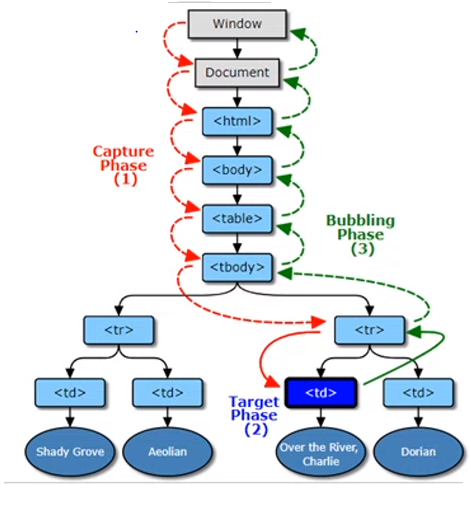
\includegraphics[height=5cm]{../lezione17/img1.PNG}
\end{center}
Ci sono degli eventi che hanno una gestione standard da parte del browser, il metodo preventDefault() può essere usato per cancellare il comportamento di default associato all'evento (es. form, anchor).\newline
A volte può essere utile simulare l'interazione di un utente, cioè programmare lo scatenamento di un evento.\newline
\newline